\documentclass[12pt,a4paper]{article}
\usepackage[utf8]{inputenc}
\usepackage{amsmath, amssymb, amsfonts}
\usepackage{geometry}
\geometry{margin=2.5cm}
\usepackage{hyperref}
\usepackage{pgfplots}
\usepackage{fancyhdr}
\usepackage{graphicx}
\usepackage{listings}
\usepackage{listing}
\usepackage{titlesec}
\titleformat{\section}
  {\normalfont\Large\bfseries\centering}  % Format: font size, bold, centered
  {\thesection}{1em}{}
\pagestyle{fancy}
\pgfplotsset{compat=1.18}
\fancyhead{}
\fancyfoot{}
\title{Ricerca Operativa}
\author{}
\date{}
\fancyhead[L]{Gabriele Perna}          % Left side
\fancyhead[C]{Ricerca Operativa}     % Center
\fancyhead[R]{2026/2027}             % Right side
\fancyfoot[C]{\thepage}           % Page number in the center of footer
\let\oldsection\section
\renewcommand{\section}{\clearpage\oldsection}

\begin{document}

\maketitle
\tableofcontents

\section{Introduzione}

\paragraph{Corso E-Learning:} \href{https:/elearning.di.unipi.it/course/view.php?id=1115}{Ricerca Operativa}\\\\
La \textbf{ricerca operativa} è la disciplina che si occupa di modellizzazione e risoluzione di problemi decisionali complessi con metodologie matematiche, dalla statistica all'informatica.\\
Il processo è complesso e non lineare.
\paragraph{Ottimizzazione:} ricerca del modo migliore per svolgere un azione, concetto importante della ricerca operativa. Tale concetto nasce durante la Seconda Guerra Mondiale, infatti la ricerca operativa nasce dallo studiare l'ottimizzazione di strategie militari.\\\\
Alcuni esempi di applicazioni della ricerca operativa:
\begin{itemize}
    \item Scheduling negli aereoporti per merce
    \item Problema dei sette ponti
    \item Routing dei dati
\end{itemize}

\section{Processo decisionale}
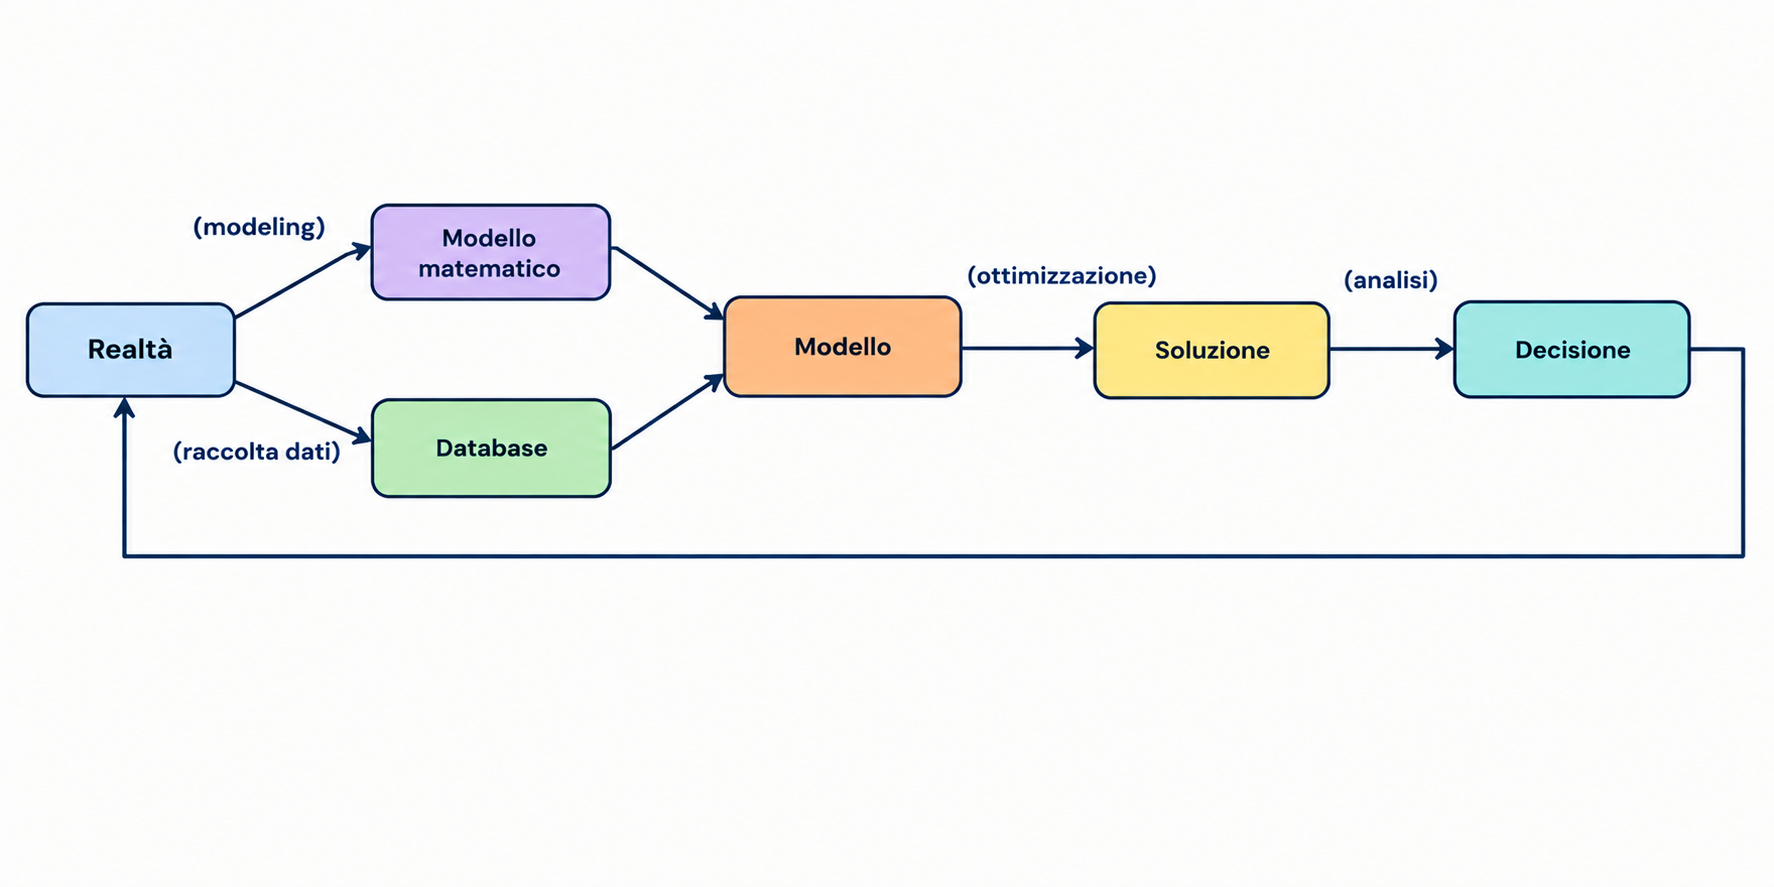
\includegraphics[width=\textwidth]{images/Diagram.png}

\section{Modelli di ottimizzazione}
Un \textbf{modello di ottimizzazione} è una rappresentazione matematica di un problema decisionale.\\
Un modello tale serve a risolvere un problema di ottimizzazione e per farlo utilizza questi:
\begin{itemize}
    \item \textbf{Funzione Obiettivo:} rappresenta ciò che vogliamo massimizzare o minimizzare (profitto, produzione...)
    \item \textbf{Variabili decisionali:} incognite del modello
    \item \textbf{Vincoli:} rappresentano le limitazioni del problenma, come il budget.
    \item \textbf{Parametri:} valori fissi, influenzano funzione obiettivo e vincoli ma non possono essere modificati.
\end{itemize}

\subsection{Programmazione lineare e lineare intera}
I nostri modelli devono essere lineari.
\paragraph{Programmazione lineare:} se i vincoli e la funbzione obiettivo sono lineari e le variabili sono continue.
\paragraph{Programmazione lineare intera:} se i vincoli e la funzione obiettivo sono lineari e alcune delle variabili sono discrete (o \textbf{intere}).\\\\
Nei nostri modelli non si può:
\begin{itemize}
    \item Dividere o moltiplicare per variabili
    \item Utilizzare valori assoluti
\end{itemize}
Si possono solo utilizzare somme e moltiplicazioni o divisioni per parametri.

\subsection{Pianificazione della produzione (esempio)}
Osserviamo adesso un problema d'esempio per apprendere come trovare un modello di ottimizzazione e quindi una soluzione ottimizzata.
\subsubsection{Descrizione del problema}
La società Pintel deve pianificare la produzione della sua fabbrica di microprocessori. L'azienda possiede due diverse linee di prodotti: processori Pintium, venduti a 500 euro, ed i Coloron, venduti a 200 euro perche meno potenti, destinati ai consumer semplici.\\
L'impianto è in grado di realizzare 3000 "wafer" alla settimana, su ogni wafer trovano posto 500 coloron oppure 300 Pintium.\\
La resa di un wafer dipende dal tipo di processore:
\begin{itemize}
    \item Pintium: $50\%$
    \item Coloron: $60\%$
\end{itemize}
Ogni settimana si può mettere sul mercato un massimo di $400.000$ unità per evitare il calo dei prezzi per i Pintium, $700.000$ per i Coloron invece.\\
Si vuole capire quale quantità di ciascun modello bisonerebbe produrre settimanalmente per massimizzare il profitto.
\subsubsection{Inizializzazione}
Iniziamo con la preparazione dei nostri dati, vediamo le variabili:
\begin{itemize}
    \item $X_P$: numero di processori Pintium.
    \item $X_C$: numero di processori Coloron.
\end{itemize}
La funzione obiettivo è:
\[
maxZ = 500X_p + 200X_C
\]
I vincoli sono:
\[
\begin{cases}
    0 \leq X_P \leq 400.000\\
    0 \leq X_C \leq 700.000\\
    \frac{X_P}{300 \cdot 0,5} + \frac{X_C}{500 \cdot 0,6} \leq 300
\end{cases}
\]

\subsubsection{Traduzione in grafico e soluzione}
Per disegnare il grafico corrispondente inanzitutto è consigliato semplificare i dati comprimendoli (per esempio quantità di centinaia o migliaia).\\
Bisogna rappresentare i vincoli e ridurre il dominio, trovando lo \textbf{spazio soluzione}.\\
Una volta fatto questo, bisogna massimizzare la funzione obiettivo con l'utilizzo del gradiente, in questo caso:
\[
\nabla z = (500,200)
\]
La soluzione consiste nell'ultimo punto in cui il gradiente, scorrendo verso destra, rimane nel dominio.
\end{document}